\newpage

\section{In Chapter 3, a formula is given to simulate $\text{Be}(\alpha, \beta)$ from the uniform distribution, given that both parameters $\alpha$ and $\beta$ are natural numbers (and not equal to 0). Implement this transformation method algorithm and apply it to simulate 15,000 values of a $\text{Be}(3, 9)$ distribution.} \label{sec:4}

% When both shape parameters $\alpha$ and $\beta$ of a Beta distribution are natural numbers, a special transformation method allows us to simulate samples using uniform random variables. This method relies on a probabilistic identity involving the logarithm of uniforms.

\subsubsection*{Theoretical background}

Let $U_j \sim \mathcal{U}[0, 1]$ be i.i.d. uniform random variables. Then, as shown in chapter 3 of the lecture:

\begin{equation}
X = \frac{ \sum_{j=1}^{\alpha} -\log(U_j) }{ \sum_{j=1}^{\alpha + \beta} -\log(U_j) } \sim \text{Be}(\alpha, \beta), \quad \text{for } \alpha, \beta \in \mathbb{N}
\end{equation}

This transformation is numerically more stable than working directly with products of uniforms, especially when $\alpha$ or $\beta$ is large.

\subsubsection*{Simulation and results}

To simulate 15,000 values from $\text{Be}(3, 9)$:
\begin{enumerate}
    \item Generate a $15{,}000 \times 12$ matrix of $U_{ij} \sim \mathcal{U}[0,1]$.
    \item Compute $S_3 = \sum_{j=1}^{3} -\log(U_j)$ and $S_{12} = \sum_{j=1}^{12} -\log(U_j)$ for each sample.
    \item Return the ratio $X = S_3 / S_{12}$.
\end{enumerate}

\begin{figure}[H]
    \centering
    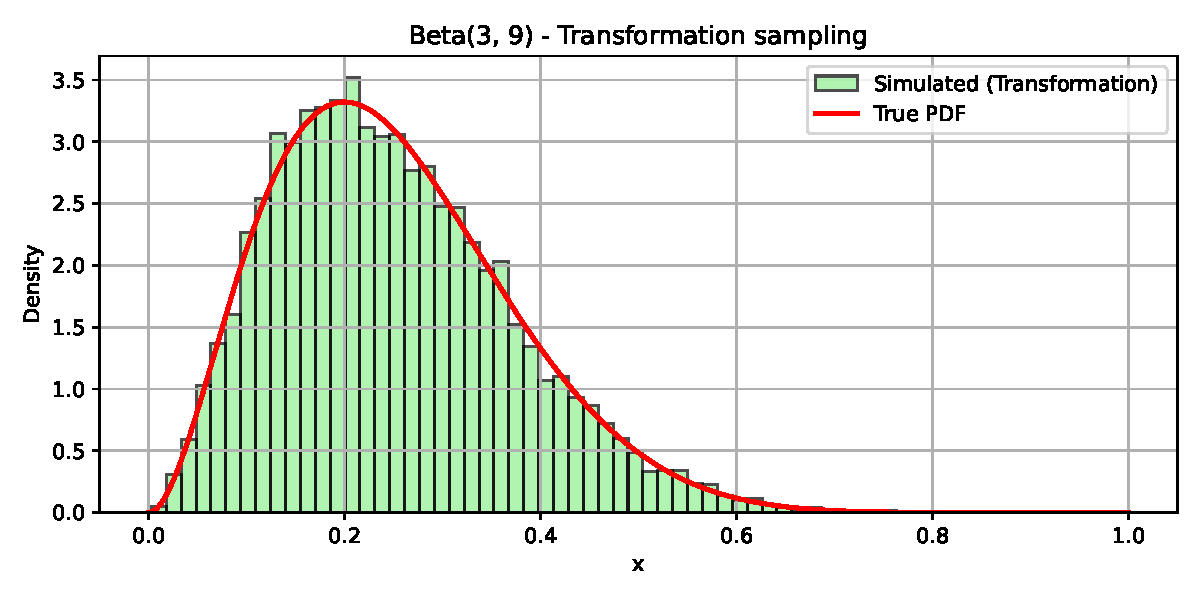
\includegraphics[width=0.7\textwidth]{resources/figures/q3-beta_transformation_sampling.pdf}
    % \caption{Histogram of 15,000 samples from $\text{Be}(3, 9)$ using the transformation method (green) compared to the true density (red).}
    \noskipcaption{Histogram of 15,000 samples from $\text{Be}(3, 9)$ using the transformation method.}
    \label{fig:beta_transform}
\end{figure}

As shown in Figure~\ref{fig:beta_transform}, the simulated samples closely follow the theoretical $\text{Be}(3, 9)$ density. The transformation method based on uniform variables offers an accurate and efficient approach when the shape parameters are integers.

% \subsubsection*{Conclusion}

% The log-transformation method provides a simple and robust way to simulate Beta distributions with integer parameters using only uniform random variables. It avoids the numerical instability of multiplicative methods and yields excellent agreement with the true distribution.




% ---

% The method that we have seen in Chapter 3 to simulate a beta distribution is the following expression:
% \[
% Y = \frac{\sum_{j=1}^{\alpha} \log(U_j)}{\sum_{j=1}^{\alpha} \log(U_j) + \sum_{j=1}^{\beta} \log(U_j)} \sim \text{Be}(\alpha, \beta)
% \]

% If we ensure that the $U_j$ are i.i.d.\ and drawn from a uniform distribution between 0 and 1 and $\alpha$, $\beta \in \mathbb{N}$, which is the case for a beta distribution, this formula is therefore usable.

% \begin{figure}[h]
%     \centering
%     % \includegraphics[width=0.7\textwidth]{your-figure-file.pdf} % Replace with actual file
%     \caption{Sample of random values for a beta distribution using the formula of Chapter 3.}
%     \label{fig:beta-simulation}
% \end{figure}

% This clearly illustrates the feasibility of using the formula seen in Chapter 3 to sample random values of a beta distribution.
